\documentclass[handout, aspectratio=169, 10pt, ngerman]{beamer}
\usepackage[utf8]{inputenc}

\usepackage{pgfpages}

\mode<handout>{%
    \pgfpagesuselayout{2 on 1}[a4paper]
    \setbeameroption{show notes}
}

\AtBeginSection[]{
  \begin{frame}[standout]
  \vfill
  \centering
  \begin{beamercolorbox}[sep=8pt,center,shadow=true,rounded=true]{title}
    \usebeamerfont{title}\insertsectionhead\par%
  \end{beamercolorbox}
  \vfill
  \end{frame}
}

%%%%%%%%%%%%%%%%%%%%%%%%%%%%%%%%%%%%%%%%%%%%%%%%%%%%%%%
% General preamble
%%%%%%%%%%%%%%%%%%%%%%%%%%%%%%%%%%%%%%%%%%%%%%%%%%%%%%%
\usetheme{reisefuhrer}
\graphicspath{{../../resources/}}

\institute{Reiseführer Mathematik}
\logo{\includegraphics[height=.5cm]{images/general/logo.pdf}}

%%%%%%%%%%%%%%%%%%%%%%%%%%%%%%%%%%%%%%%%%%%%%%%%%%%%%%%
% Presentation specific preamble
%%%%%%%%%%%%%%%%%%%%%%%%%%%%%%%%%%%%%%%%%%%%%%%%%%%%%%%
\title{Reiseführer Mathematik}
\subtitle{Mathematik geht auch einfach}
\author{TH}
\date{\today}
\titlegraphic{\includegraphics{images/math/faultier-balkenwaage.jpg}}

\usepackage{csquotes}
\usepackage{relsize}
\usepackage{tabularx}

\usepackage{tikz}
\usetikzlibrary{positioning, scopes, shadows.blur, shapes.geometric}
%
%%%%%%%%%%%%%%%%%%%%%%%%%%%%%%%%%%%%%%%%%%%%%%%%%%%%%%%

\begin{document}
\begin{frame}[plain,noframenumbering]
    \maketitle
    \note{
        Willkommen zum Reiseführer Mathematik. In diesem Video stellen wir Dir den Reiseführer Mathematik vor, sodass Du am Ende weist, was der Reiseführer Mathematik ist und wie er Dir helfen kann, Mathematik nachhaltig zu verstehen.
    }
\end{frame}
\begin{frame}
    \note{
        Die häufigste Frage, die wir von unseren Mitschülern in unserer eigenen Schulzeit gehört haben -- und die Dich sicher auch schon beschäftigt hat -- ist: \enquote{Warum müssen wir Mathematik überhaupt lernen?} Wir aber behaupten, dass das die falsche Frage ist. Sie impliziert scheinbar schon, dass man von außen gezwungen wird, Mathematik zu lernen. Das ist zwar sicher nicht ganz falsch. Stattdessen möchten wir aber die Frage stellen und beantworten, \textbf{warum} Mathematik interessant ist.
    }
    
    \begin{tikzpicture}[overlay, remember picture]
        %\fill[green!20!rm@highlight!20] (current page.north west) |- (current page.south) |- cycle;
        %\fill[blue!20!rm@highlight!20] (current page.north) |- (current page.south east) |- cycle;
        \node[draw, fill=white, ellipse, align=center, blur shadow={shadow blur steps=5}] (C) at (current page) {Warum ist Mathe\\interessant?};
        %\node[align=center] at (1, 1) {Mathe ist Teil\\der Schulbildung};
    \end{tikzpicture}

    \note{
        Je mehr man sich mit Mathematik beschäftigt, desto mehr wird einem auffallen, dass man sie sich sehr gut als eine eigene Sprache vorstellen kann, die einem eine analytische und strukturierte Herangehensweise für vielerlei Probleme eröffnet. Das bedeutet aber, dass Mathematik kein alleinstehendes Fach ist. Stattdessen findet sie Anwendung in und ist notwendig für alle möglichen Fächer und Berufe.
        
        Gerade wenn es um so subjektive Fragen wie "Interesse" geht, sind Fakten aber keine gute Antwort. Deswegen möchten wir Dir mit dem Reiseführer Mathematik zeigen, dass Mathematik nicht nur Formeln auswendig lernen und Rechnen ist. Auch wenn dich nicht jedes einzelne Thema begeistert, wird sicherlich viel spannendes dabei sein.
    }
\end{frame}
\begin{frame}{Reiseführer Mathematik}
    \begin{center}
        \begin{tabularx}{.7\linewidth}{>{\centering\arraybackslash}X@{\hspace{.7cm}}>{\centering\arraybackslash}X}
            \textbf{Frontalunterricht} & \textbf{Flipped Classroom}\\
            \includegraphics[width=\linewidth]{example-image} & \includegraphics[width=\linewidth]{example-image}
        \end{tabularx}
    \end{center}

    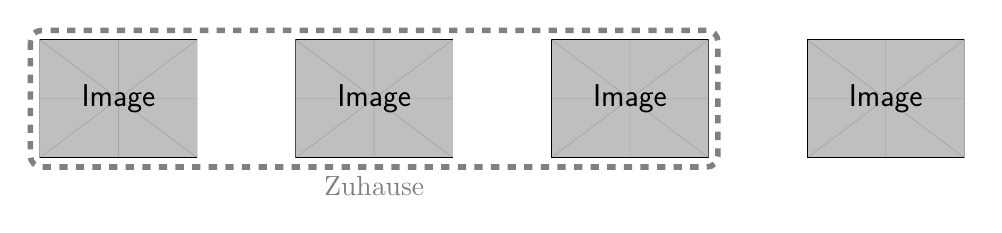
\begin{tikzpicture}[]
        {[local bounding box=home]
            \node (book) {\includegraphics[width=2cm]{example-image}};
            \node[right=of book] (videos) {\includegraphics[width=2cm]{example-image}};
            \node[right=of videos] (vb) {\includegraphics[width=2cm]{example-image}};
        }
        \node[right=of vb] (ab) {\includegraphics[width=2cm]{example-image}};
        \draw[dashed, gray, line width=2pt, rounded corners] (home.north west) rectangle (home.south east);
        \node[anchor=north, gray] at (home.south) {Zuhause};
    \end{tikzpicture}
    
    \note{\smaller
        Um Dir Mathematik möglichst gut beizubringen, verfolgen wir das Flipped Classroom Konzept. Ein Problem mit traditionellem Frontalunterricht ist, dass Schüler im Klassenzimmer still sitzen und zuhören müssen und zuhause mit Hausaufgaben das gelernte Anwenden sollen. Dabei ist es \textbf{gerade} beim Üben, dass Fragen und Unsicherheiten auftreten, die man am besten direkt mit Mitschülern und Lehrern besprechen möchte. Flipped Classroom dreht das genau um: Zuhause wird neues Wissen erarbeitet und im Klassenzimmer zusammen mit den Mitschülern und dem Lehrer geübt.

        
        Unser Lehrkonzept besteht grundlegend aus vier Komponenten:
        \begin{itemize}
            \item Einem Lehrbuch, das zuhause gelesen wird, um den Stoff vorzubereiten
            \item Lehrvideos, die ihr euch freiwillig zusätzlich anschauen könnt, um wichtige Passagen nochmal anders erklärt zu bekommen
            \item Vorbereitungsblätter
            \item und zuletzt Aufgabenblöcke, die im Unterricht bearbeitet werden
        \end{itemize}
        Dabei sind Vorbereitungsblätter sehr kurze Aufgabenblätter, die ihr ausfüllt während ihr das Buch lest. Sie sollen euch helfen, das Buch aufmerksam zu lesen. Es passiert jedem mal, dass man die Gedanken wandern lässt, wenn man ein Buch liest -- und die Vorbereitungsblätter haben als einzige Aufgabe lediglich, euch zu ermöglichen, aktiv zu lesen (insbesondere sind sie nicht dafür da, zu überprüfen, ob ihr das Buch gelesen habt). Die Aufgaben auf den Vorbereitungsblättern könnt ihr immer direkt mit dem Wissen aus dem Buch lösen. Dafür geben wir euch eine Kein-Grübeln-Notwendig-Garantie.
    }
\end{frame}
\begin{frame}{Vorteile}
    
    \begin{itemize}
        \item Nur eine Hausaufgabe: ein paar Seiten lesen
        \begin{itemize}
            \item Weniger Leistungsdruck
            \item Fester Arbeitsaufwand
        \end{itemize}
        \item Unser Ziel: Verständnis statt Faktenwissen
        \begin{itemize}
            \item Weniger Stress vor Klassenarbeiten
            \item Bessere Noten
        \end{itemize}
        \item Spaß an Mathe!
    \end{itemize}
    \textcolor{red}{Hier fehlen Bilder}
    
    \note{\smaller
        Welche Vorteile hat das Flipped Classroom Konzept nun aber konkret für Dich als Schüler? Oder bedeutet es 'gar mehr Arbeit? Es mag auf den ersten Blick so wirken, als hättest du wesentlich mehr Hausaufgaben auf, aber das ist nicht der Fall.

        Deine Hausaufgaben mit Flipped Classroom sind wesentlich geregelter. Anstatt zuhause Aufgaben rechnen zu müssen und im schlimmsten Fall an ihnen zu verzweifeln und Stunden zu verschwenden, brauchst du lediglich ein paar Seiten des Buches in Vorbereitung auf die nächste Unterrichtsstunde lesen. Die Aufgaben auf dem Vorbereitungsblatt sollen dabei weder viel Zeit in Anspruch nehmen noch dazu dienen, zu überprüfen, ob du das Buch tatsächlich gelesen hast. Stattdessen helfen sie Dir, aktiv das Buch zu lesen und dich selbst zu überprüfen. Es ist auch nicht Deine Aufgabe, alles auf Anhieb zu verstehen. Das Üben -- und damit das Lernen -- geschieht anhand der Aufgabenblöcke im Klassenzimmer.

        Das Buch ist zusammen mit dem Flipped Classroom Konzept darauf ausgelegt, Dir Verständnis für die Mathematik zu vermitteln. Was man einmal verstanden hat, vergisst man nicht so schnell wieder, sodass langes Büffel für eine Klassenarbeit, weil man die Hälfte des Stoffes wieder vergessen hat, passé ist.

        Vor Allem hoffen wir aber, dass wir dir mit dem Reiseführer Mathematik zeigen können, dass Mathematik auch Spaß machen kann und hoffen, dein Interesse für zumindest ein paar der Themen wecken zu können. Denn wenn Dir das Lernen Spaß macht, ist Mathematik am einfachsten.
    }
\end{frame}
\begin{frame}{Wie bin ich erfolgreich?}
    \begin{itemize}
        \item Gewissenhaft arbeiten
        \item Offen sein für neue Themen
    \end{itemize}
    \vfil
    \begin{center} % Faultier, dass an einem Kartenhaus eine Karte weg nimmt, sodass es wackelt
        \includegraphics[width=.4\linewidth]{example-image}
    \end{center}
    \note{
        Flipped Classroom kann aber nur funktionieren, wenn man sich sich daran hält. Das Buch sollte aufmerksam gelesen werden. Du musst und wirst nicht alles auf Anhieb verstehen aber wenn Du das Buch nicht gewissenhaft liest, funktioniert das Konzept nicht. Die Aufgabenblöcke sind auch nicht dafür da, dass jeder am Ende das richtige Ergebnis aufgeschrieben hat. Nutze die Chance, um Aufgaben auch selbständig lösen zu können.

        Sei offen für neue Themen. Wenn man das erste Mal ein neues mathematisches Konzept kennen lernt, fühlt es sich oft so an als wäre es zu schwer. Versuch' zuerst, die Übungsaufgaben zu neuen Themen zu üben und stempel sie nicht als zu schwer ab.
        
        Wage gerne einen Blick über den Tellerrand hinaus und versuch dich auch an Knobelaufgaben. Sie nicht zu schaffen ist keine Schande aber alleine der Versuch übt das Verständnis ungemein.
    }
\end{frame}

\begin{frame}{Anleitung}
    \begin{center}
        \includegraphics[height=6cm]{example-image}
    \end{center}
    \note{
        
    }
\end{frame}
\begin{frame}{Ein typischer Schultag}
    \note{
        
    }
\end{frame}
\begin{frame}{Das Buch}
    
\end{frame}
\begin{frame}{Vorbereitungsblätter}
    
\end{frame}
\begin{frame}{Aufgabenblöcke}
    
\end{frame}
\begin{frame}{TODO: OUTRO}
    \note{
    
    }
\end{frame}
\end{document}